\documentclass[11pt,spanish]{article}

\usepackage[a6paper, landscape,
	left=1cm, top=1cm, right=1cm, bottom=1.5cm
]{geometry}
%\usepackage[a4paper, margin=3cm]{geometry}
\usepackage{babel}
\usepackage{xltxtra}
\usepackage{grid-system}
\usepackage{multicol} % simpler than grid for lots of cases
\usepackage{hyperref}
\usepackage{xcolor}
\usepackage{graphicx}
\usepackage[export]{adjustbox}
\usepackage{fancyhdr}
\usepackage{listings}

\setmainfont{Comic Sans MS}
%\setmathfont{eulervm}
%\lstset{basicstyle=\footnotesize\ttfamily}
\lstset{basicstyle=\footnotesize\setmainfont{DejaVu Sans Mono}}

\definecolor{verletblue}{HTML}{487AD8}
\definecolor{verletgreen}{HTML}{37DE88}
\definecolor{verletcyan}{HTML}{1AFBFF}

\fancyhead{}
\fancyfoot{}
\fancyfoot[RO]{{\footnotesize \thepage\ de\ \pageref*{lastpage}}}
\renewcommand{\headrule}{}
%\renewcommand{\footrule}{\vbox to 0pt{\hbox to\headwidth{\dotfill}\vss}}
% XXX should find way to use only one right aligned rule...
\renewcommand{\footrule}{{\footnotesize \rule{\textwidth - 5ex}{0pt}\rule{5ex}{1pt}\vss}}
\pagestyle{fancy}

\newcommand{\fr}[1]{%
	\begin{flushright}
		#1
	\end{flushright}
}
%row space
\newcommand{\rowsp}[1][1em]{\vspace{#1}}
\newcommand{\hone}[1]{{\rowsp[0.3em]\noindent\Large #1 \rowsp[0.3em]}}
\newcommand{\htwo}[1]{{\rowsp\noindent\large #1 \rowsp}}
\newcommand{\htworuler}[1]{{%
	\rowsp\noindent\Large #1%
	\\ {\color{verletgreen}\noindent\rule{\textwidth + 2em}{0.5em}}\rowsp%
}}
\newcommand{\hthree}[1]{{\rowsp\noindent\large #1 \rowsp[0.5em]}}
\newcommand{\hfour}[1]{{\rowsp\large #1 \rowsp[0.5em]}}
\newcommand{\for}[1]{{#1 \rowsp}}
\newcommand{\signline}{\rule{\textwidth}{1pt}}
\newcommand{\emptycell}[1][1]{\begin{Cell}{#1}\ \end{Cell}}

%=======================
% specific to presentations
%\newcommand{\myitm}{aoeuaeou}
\newcommand{\myitm}[1]{\begin{itemize}#1\end{itemize}}

\newcommand{\mydesc}[1]{%
	\begin{description}
	\setlength\itemsep{0em}%
	#1
	\end{description}
}
\newcommand{\pros}{\item[pros:]}
\newcommand{\cons}{\item[cons:]}

\setlength{\parindent}{0pt}
\setlength{\parskip}{1ex plus 0.5ex minus 0.2ex}
%=======================

%\renewcommand{\emph}[1]{\emph{#1}}

\title{Postperf: performance en PostgreSQL}
\author{Abel Camarillo $<$acamari@verlet.org$>$}

\begin{document}

\maketitle
\thispagestyle{empty}

\newpage

\hone{Agenda}

\myitm{
	\item ¿Quién soy?
	\item ¿Qué es PostgreSQL?
	\item Cómo medir tiempos actuales
	\item Modelo de capas propuesto
}

\newpage
\hone{¿Quién soy?}
\begin{Row}
\begin{Cell}{2}
\myitm{
	\item Desarrollador de software desde el 2008 - OpenBSD, perl, C, sh, js
	\item Lead developer en Neuroservices Communications durante 6 años.
	\item Desarrollador freelance desde el 2015 - Verlet.
	\item Maintainer de 21 paquetes en el árbol oficial de OpenBSD -
	\href{http://openports.se/bbmaint.php?maint=acamari@verlet.org}{
	      http://openports.se/bbmaint.php?\textbackslash{} maint=acamari@verlet.org}
	\item Interés en UNIX, poesía, $\sim$arte$\sim$, cocina, etc...
}
\end{Cell}

\begin{Cell}{1}
\ \\ %XXX so image hasn't its bottom to baseline
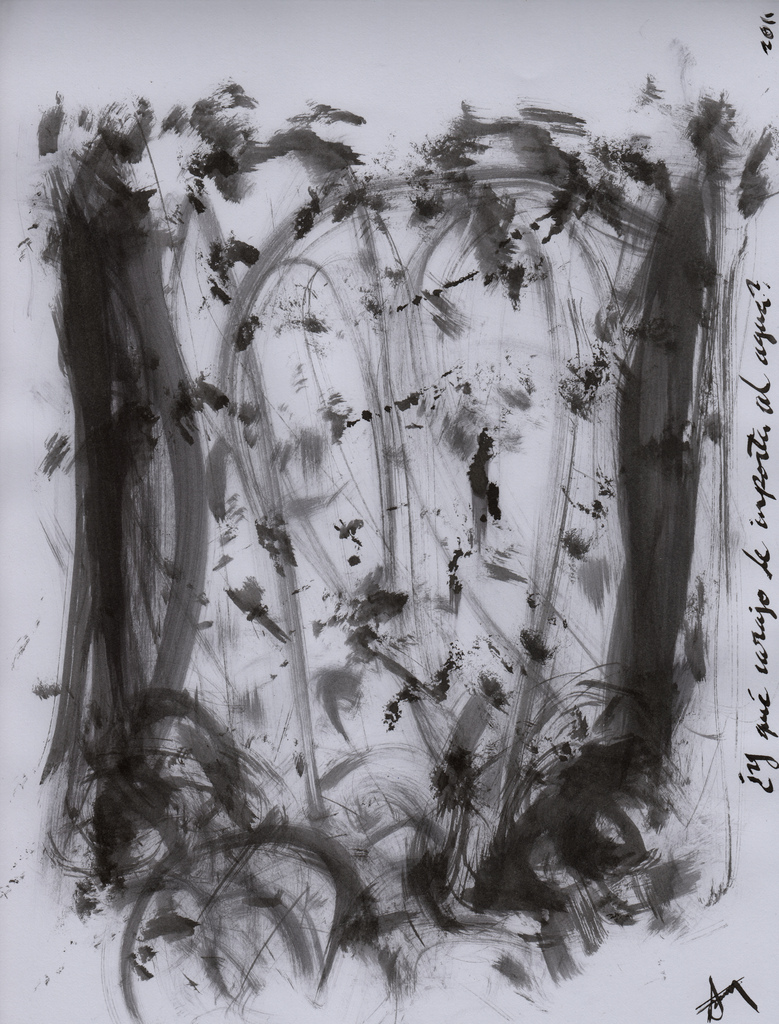
\includegraphics[width=\textwidth]{img/carajo}
\fr{ {\tiny ¿Y qué carajo\\
le importa al agua? - 2011} }
\end{Cell}

\end{Row}


\newpage

\hone{¿Qué es PostgreSQL?}

\myitm{
	\item También llamado sólo postgres.
	\item De UCB - berkley, basado en Ingres (1985), licencia BSD-like
	\item Features avanzados: gist, geqo, sp-gist, gin
	\item Altamente personalizable: 
	\myitm{
		\item C, SQL, PL/pgSQL, PL/Perl, PL/Lua, PL/Python, PL/V8, PL/sh,
			etc...
		\item FDW - foreign data wrappers (conexiones a otras DB)
		\item Publish/suscribe async - LISTEN/NOTIFY;
	}
	\item JSON nativo: store, búsquedas indexadas(!), ¿web scale$\sim$?
	\item intersección de geometrías, rangos - indexada
}


\newpage
\hone{Cómo medir tiempos actuales}

\htwo{psql \textbackslash timing}

\begin{multicols}{2}
\begin{lstlisting}
$ psql -U postgres  db      
psql (9.4.1)
Type "help" for help.

db=# \timing on
Timing is on.
db=# select 1;
 ?column? 
----------
        1
(1 row)

Time: 1.641 ms
db=# 
\end{lstlisting}

\columnbreak

\mydesc{
	\pros rápido, disponible para TODOS los queries.
	\cons el tiempo incluye latencia de red y procesamiento del cliente.
}
\end{multicols}

\newpage %===============
\hone{Cómo medir tiempos actuales}

\htwo{EXPLAIN ANALYZE}

\begin{lstlisting}
db=# explain analyze select 1;
                                     QUERY PLAN                                     
------------------------------------------------------------------------------------
 Result  (cost=0.00..0.01 rows=1 width=0) (actual time=0.003..0.004 \
					   	  rows=1 loops=1)
 Planning time: 0.031 ms
 Execution time: 0.036 ms
(3 rows)
db=# 
\end{lstlisting}

\mydesc{
	\pros excluye i/o cliente, incluye planeación y ejecución, granularidad
	\cons no disponible en todos los queries (pero sí select/ins/upd/del)
}

\newpage %===============
\hone{Cómo medir tiempos actuales}

\htwo{pgbadger}

De \url{http://pgbadger.darold.net/samplev7.html#time-consuming-queries}

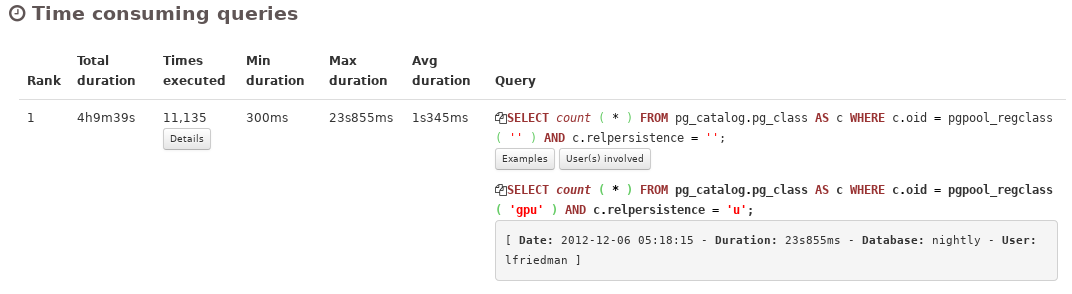
\includegraphics[width=\textwidth]{img/pgbadger-tm1}

\newpage %===============
\hone{Cómo medir tiempos actuales}
\htwo{pgbadger}

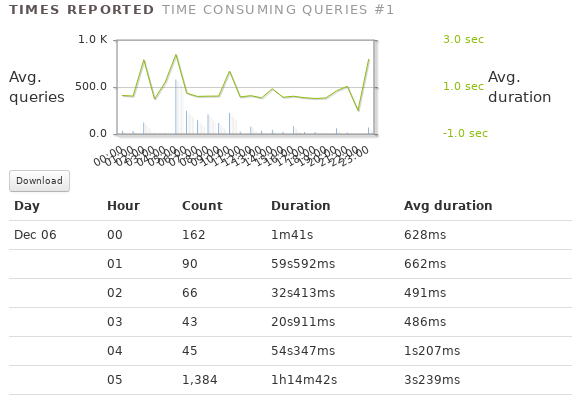
\includegraphics[scale=0.4]{img/pgbadger-tm2}

\newpage %===============
\hone{Cómo medir tiempos actuales}

\htwo{pgbadger}

Configuración pg para pgbadger:

\begin{lstlisting}
# -1 is disabled, 0 logs all statements
log_min_duration_statement = 50 

log_checkpoints = on
log_connections = on
log_disconnections = on
log_line_prefix = '%t [%p]: db=%d,user=%u,app=%a,client=%h '
		# special values:
		#   %a = application name
		#   %u = user name
		#   %d = database name
		#   %r = remote host and port
		#   %h = remote host
		#   %p = process ID
		#   %t = timestamp without milliseconds
		#   %m = timestamp with milliseconds
		#   %n = timestamp with milliseconds (as a Unix epoch)
		#   %i = command tag
		#   %e = SQL state
		#   %c = session ID
		#   %l = session line number
		#   %s = session start timestamp
		#   %v = virtual transaction ID
		#   %x = transaction ID (0 if none)
		#   %q = stop here in non-session
		#        processes
		#   %% = '%'
		# e.g. '<%u%%%d> '
log_lock_waits = on                     # log lock waits >= deadlock_timeout
log_temp_files = 0	# -1 disables, 0 logs all temp files
\end{lstlisting}


\newpage %===============
\hone{Cómo medir tiempos actuales}

\vspace{\stretch{1}}
\begin{center}
\htwo{Cualquier mecanismo que tenga su lenguaje/aplicación}
\end{center}
\vspace{\stretch{1}}

\newpage %===============
\hone{Modelo de capas propuesto}

Se propone el siguiente orden para analizar problemas de rendimiento,
no necesariamente se tienen que cumplir todas las capas...

\myitm{
	\item \emph{Capa 0}: física/hardware/fierros: beneficios $N$
	\item \emph{Capa 1}: postgres.conf: beneficios $N$
	\item Capas SQL:
	\myitm{
		\item \emph{Capa 2}: EXPLAIN/EXPLAIN ANALYZE
		\item \emph{Capa 3}: índices: beneficios 
			$O(\log N), O(n \log N), O(<N)$
		\item \emph{Capa 4}: \emph{query}: beneficios
			$O(\log N), O(n \log N), O(\ll N)$
	}
}

\newpage %===============
\hone{Modelo de capas propuesto: capa 0 física}

Al trabajar en esta capa:
\mydesc{\pros no hay que modificar la aplicación
	\cons no esperar beneficios mayores que aritméticos,
		en el mejor de los casos}

\mydesc{
	\item[CPU:] más ghz, más cores, menos threads, más cpus, más cache.
	\mydesc{
		\pros beneficios lineales, cpu doble de rápido, db doble de rápida.
		\cons beneficios lineales, costo no lineal$\sim$
	}
}

\newpage %===============
\hone{Modelo de capas propuesto: capa 0 física}
\mydesc{
	\item[RAM:] más ram, más rápida, doble/quádruple de canales - dual chan vs quad
			chan (Intel Core i7-5960X,
				AMD Opteron 6300-series 'Abu Dhabi' (32 nm), etc)
	\mydesc{
		\pros beneficios lineales
		\cons beneficios lineales, costo no lineal$\sim$, pocos
			órdenes de magnitud (x2, x4, x8, ... x16, x32)
	}
}


\newpage %===============
\hone{Modelo de capas propuesto: capa 0 física}

\mydesc{
	\item[HDD (el cuello de botella común):] más discos en arreglos RAID
	\mydesc{\pros beneficios lineales, más órdenes de magnitud
		(x2, x4, ..., x128, x256), redundancia, datasets más grandes
		(cientos de TB)
		\cons costo lineal + mantenimiento RAID, bottleneck se mueve a 
			bus de datos, PCIev2 (4GBytes/s), PCIev3 (8GBytes/s)
	}
	\item[HW RAID:]
		\mydesc{\pros mucho más rápido, y robusto, libera CPU,
		topologías versátiles (discos duros por fibra a km del data
		center), independiente de SO - movible entre SOs,
			soporte de boot, transparente al SO
			\cons más caro - tarjetas caras (>1000USD), cableado caro y de poco 
				acceso, si la tarjeta falla, debe reemplazarse 
				por otro modelo idéntico - o no se garantiza
				nada, incompatibilidad entre proveedores,
				pobre documentación.
		}

}
		
\newpage %===============
\hone{Modelo de capas propuesto: capa 0 física}
\mydesc{
	\item[SW RAID:]
		\mydesc{\pros barato, soporte de disciplinas de cifrado, 
				si fallan todos los componentes menos los discos
				se pueden mover a otra computadora
			\cons sin soporte boot (¿Linux?, OpenBSD sí soporta),
				incompatible entre SO, más carga al SO (CPU+RAM)
		}
}

\newpage %===============
\hone{Modelo de capas propuesto: capa 1 postgresql.conf}

Archivo principal de configuración de postgres en un cluster (instancia de
postgres).

\begin{lstlisting}
$ cd /tmp/
$ mkdir pg
$ initdb -D pg -E UTF-8 --no-locale -U postgres
[..]
$ ls -alsh pg/postgresql.conf
44 -rw-------  1 acamari  wheel  20.8K Oct 15 07:26 pg/postgresql.conf
$ 
\end{lstlisting}

Al trabajar en esta capa:
\mydesc{\pros No hay que modificar la aplicación, hay buena documentación,
		simple
	\cons beneficios aritméticos, más complejo  que meter fierros, más barato}

\newpage %===============
\hone{Modelo de capas propuesto: capa 1 postgresql.conf}

A modificar:
\mydesc{
	\item[mem:] \ 
	\myitm{
		\item \lstinline!shared_buffers(128MB)!: global
		\item \lstinline!temp_buffers(8MB)!: por sesión
			(CREATE TEMP TABLE)
		\item \lstinline!work_mem(4MB)!: por sesión (\lstinline!SELECT
		... ORDER BY ...!,

		\lstinline!SELECT ... WHERE col_con_indice_hash = const!)
	}
	\mydesc{
		\pros i/o a disco menos frecuente
		\cons más uso de ram por sesión  en algunos casos aunque no
		hagan nada, menos usuarios a la vez}
}

\newpage %===============
\hone{Modelo de capas propuesto: capa 1 postgresql.conf}

\mydesc{
	\item[costos de planner:] éstos se usan para decidir cuándo
	hacer seq scan vs index scan
	\myitm{
		\item \lstinline!seq_page_cost(1.0)!: aumentando: promueve idx
		scan, reduciendo: promueve seq scan
		\item \lstinline!random_page_cost(4.0)!: lo opuesto$\sim$
	}

	Promover index scan:
	\mydesc{
		\pros beneficia tiempos de ejecución dramáticamente en queries
			de alta 'selectividad' - que regresan pocos registros -
			al usar índices, complejidad $O(\log N), O(n \log N)$
		\cons genera mucha más i/o para queries de baja selectividad -
			que regresan muchos registros
	}

}

\newpage %===============
\hone{Modelo de capas propuesto: capa 1 postgresql.conf}

\mydesc{
	\item[vacumm:] proceso periódico que regresa espacio en desuso a disco.
	MVCC
	\myitm{
		\item \lstinline!vacumm_cost_limit(200)!, cuando el costo de i/o
		en vacumming sea mayor a éste, duerme por
		\lstinline!vacumm_cost_delay! milisegundos.
		\item \lstinline!vacumm_cost_delay(0 [ms])!, si es 0 no se
		duerme nunca.
	}
	\pros vacumm durmiente genera i/o a disco más distribuido - en lugar de
	picos.
	\cons si hay flujo agresivo de update/delete se acumulan 'zombies', 
		no se tienen estadísticas tan frecuentes - que puede perjudicar
		planes, promover seq scan.
}

\newpage %===============
\hone{Modelo de capas propuesto: capa 1 postgresql.conf}
\mydesc{
	\item[wal:] write ahead log: log de reconstrucción en caso de crash y
	para replicación.
	\myitm{
		\item \lstinline!checkpoint_segments(3)!, número de segmentos (de
		16MB cada uno) a cachear antes de escribir en disco y al log WAL
	}

	Aumentando:
	\pros i/o a disco menos frecuente, mejora rendimiento en picos
	\cons más tiempo de recuperación de crash (pkill -9 postgres, kernel
	panic, pérdida de energía eléctrica), probable pérdida de datos.
}

\newpage %===============
\hone{Modelo de capas propuesto: capa 2 EXPLAIN ...}

\begin{lstlisting}
db=# 
db=# create table herp (a int);
CREATE TABLE
db=# insert into herp (a) values (0), (1), (2), (3), (4), (5), (6), (7);
INSERT 0 8
db=# 
db=# explain select a from herp where a = 3;
                      QUERY PLAN                      
------------------------------------------------------
 Seq Scan on herp  (cost=0.00..40.00 rows=12 width=4)
   Filter: (a = 3)
(2 rows)

db=# \timing
Timing is on.
db=# 
db=# 
db=# 
db=# select a from herp where a = 3;
 a 
---
 3
(1 row)

Time: 0.781 ms
db=# 
db=# explain analyze select a from herp where a = 3;
                                           QUERY PLAN                                           
---------------------------------------------------------------
 Seq Scan on herp  (cost=0.00..40.00 rows=12 width=4) (actual \
	time=0.020..0.024 rows=1 loops=1)
   Filter: (a = 3)
   Rows Removed by Filter: 7
 Planning time: 0.104 ms
 Execution time: 0.176 ms
(5 rows)

Time: 0.989 ms
db=# 
db=# truncate herp; 
TRUNCATE TABLE
Time: 36.185 ms
db=# 
db=# -- insertar carga más real, 1 millón de reg
db=# insert into herp (a) select a from generate_series(1,1000 * 1000) as s(a);

INSERT 0 1000000
Time: 1399.472 ms
db=# 
db=# explain select a from herp where a = 3;
                       QUERY PLAN                       
--------------------------------------------------------
 Seq Scan on herp  (cost=0.00..17700.00 rows=1 width=4)
   Filter: (a = 3)
(2 rows)

Time: 0.811 ms
db=# 
db=# explain analyze select a from herp where a = 3;
                                             QUERY PLAN                                             
---------------------------------------------------------------
 Seq Scan on herp  (cost=0.00..17700.00 rows=1 width=4) (actual \
	time=0.036..205.402 rows=1 loops=1)
   Filter: (a = 3)
   Rows Removed by Filter: 999999
 Planning time: 0.104 ms
 Execution time: 205.452 ms
(5 rows)

Time: 206.054 ms
db=# 
db=# -- limpiar tabla e insertar 10 millones
INSERT 0 10000000
Time: 13153.689 ms
db=# 
db=# explain select a from herp where a = 3;
                       QUERY PLAN                        
---------------------------------------------------------
 Seq Scan on herp  (cost=0.00..176992.00 rows=1 width=4)
   Filter: (a = 3)
(2 rows)

Time: 0.386 ms
db=# 
db=# explain analyze select a from herp where a = 3;
                                              QUERY PLAN                                              
---------------------------------------------------------------
 Seq Scan on herp  (cost=0.00..176992.00 rows=1 width=4) (actual \
	time=1.811..2379.152 rows=1 loops=1)
   Filter: (a = 3)
   Rows Removed by Filter: 9999999
 Planning time: 0.192 ms
 Execution time: 2379.197 ms
(5 rows)

Time: 2379.840 ms
db=# 
db=# 
db=# -- limpiar tabla e insertar 100 millones
INSERT 0 100000000
Time: 203101.817 ms
db=# 
db=# 
db=# explain select a from herp where a = 3;
                        QUERY PLAN                        
----------------------------------------------------------
 Seq Scan on herp  (cost=0.00..1769912.00 rows=1 width=4)
   Filter: (a = 3)
(2 rows)

Time: 1.197 ms
db=#
db=#
db=#
db=#
db=#
db=#
db=#
db=# -- disco a 180MBps un core al 30%
db=# explain analyze select a from herp where a = 3;
                                               QUERY PLAN                                               
---------------------------------------------------------------
 Seq Scan on herp  (cost=0.00..1769912.00 rows=1 width=4) (actual \
	time=0.146..63725.876 rows=1 loops=1)
   Filter: (a = 3)
   Rows Removed by Filter: 99999999
 Planning time: 0.081 ms
 Execution time: 63725.905 ms
(5 rows)

Time: 63726.374 ms
db=# 
\end{lstlisting}

\newpage %===============
\hone{Modelo de capas propuesto: capa 3 índices}

Al trabajar en esta capa:
\mydesc{\pros no hay que modificar la aplicación, beneficios dramáticos, complejidad baja a 

	 \[O(\log n) \textrm{ o } O(n*c \log n) | c \ge 1\]

	dependiendo del tipo de índice  btree, gin, gist, sp-gist,
	hash ($O(1)$ a $O(n)$)
	
	\cons el indexado hace apreciablemente más lento (x2$\sim$) los
		insert/update/deletes debido al i/o extra, cada índice a una
		columna X gasta
		alrededor del almacenamiento en disco que ocupa la columna X en sí
		
}

\newpage %===============
\begin{lstlisting}
db=# -- añadiendo índice btree a la columna principal
db=# create index on herp (a);
CREATE INDEX
Time: 148020.907 ms
db=# 
db=# explain select a from herp where a = 3;
                                 QUERY PLAN                                 
---------------------------------------------------------------
 Index Only Scan using herp_a_idx on herp  (cost=0.57..8.59 \
	rows=1 width=4)
   Index Cond: (a = 3)
(2 rows)

Time: 3.252 ms
db=# 
db=# 
db=# 
db=# 
db=# 
db=# 
db=# -- leyendo de disco
db=# explain analyze select a from herp where a = 3;
                                                       QUERY PLAN                                                       
---------------------------------------------------------------
 Index Only Scan using herp_a_idx on herp  (cost=0.57..8.59 \
	rows=1 width=4) (actual time=32.697..32.704 rows=1 loops=1)
   Index Cond: (a = 3)
   Heap Fetches: 1
 Planning time: 0.208 ms
 Execution time: 33.379 ms
(5 rows)

Time: 34.234 ms
db=# 
db=# 
db=# 
db=# 
db=# 
db=# 
db=# 
db=# -- dato aledaño, probablemente en cache
db=# explain analyze select a from herp where a = 50;
                                                      QUERY PLAN                                                      
---------------------------------------------------------------
 Index Only Scan using herp_a_idx on herp  (cost=0.57..8.59 rows=1 \
	 width=4) (actual time=0.040..0.043 rows=1 loops=1)
   Index Cond: (a = 50)
   Heap Fetches: 1
 Planning time: 0.165 ms
 Execution time: 0.097 ms
(5 rows)

Time: 1.064 ms
db=#
db=# 
db=# 
db=# 
db=# 
db=# 
db=# 
db=# -- otra búsqueda
db=# explain analyze select a from herp where a = 50000000;
                                                      QUERY PLAN                                                      
---------------------------------------------------------------
 Index Only Scan using herp_a_idx on herp  (cost=0.57..8.59 rows=1 \
	 width=4) (actual time=1.045..1.050 rows=1 loops=1)
   Index Cond: (a = 50000000)
   Heap Fetches: 1
 Planning time: 0.191 ms
 Execution time: 1.109 ms
(5 rows)

Time: 2.020 ms
db=# 
\end{lstlisting}

\newpage %===============
\hone{Modelo de capas propuesto: capa 4 query}

En esta capa nos podemos enfocar en optimizar queries específicos,
también podemos migrar más trabajo de búsqueda de datos directo a la db -
y reducir los ciclos aplicación - net i/o - pg (de ida y vuelta)
y explotar la optimización de queries que hace postgres:

\mydesc{\item Todo en esta capa interfiere con la aplicación, hay que modificarla}

Al trabajar en esta capa:
\myitm{
	\item Migrando a db la lógica: stored procedures/funciones, SQL, PL/pgSQL;
		
	\mydesc{\pros eliminación de mucha net/io, explota el optimizador de
			queries de postgres, permite reciclar lógica entre
			aplicaciones
		\cons modificar aplicación, requiere aprender sintaxis nueva
		}

	\item Largas cadenas de selects/insert/update convertidas a un solo
		query mejora integridad de datos y no genera locking explícito
}


\newpage %===============
\hone{Modelo de capas propuesto: capa 4 query}

Errores comunes: count(*)

Genera un seq scan de toda la tabla, si sólo se quiere saber si hay registros
o no en una tabla, se sugiere:

\begin{lstlisting}
db=# explain select count(*) from herp;
                               QUERY PLAN                               
---------------------------------------------------------------
 Aggregate  (cost=1692478.00..1692478.01 rows=1 width=0)
   ->  Seq Scan on herp  (cost=0.00..1442478.00 rows=100000000 width=0)
(2 rows)

Time: 0.854 ms
db=# select count(*) from herp;
   count   
-----------
 100000000
(1 row)
Time: 27080.496 ms
db=# 
db=# explain analyze select 1 from herp limit 1;
                                                    QUERY PLAN                                                    
---------------------------------------------------------------
 Limit  (cost=0.00..0.01 rows=1 width=0) (actual time=0.035..0.037 \
	rows=1 loops=1)
   ->  Seq Scan on herp  (cost=0.00..1442478.00 rows=100000000 \
	width=0) (actual time=0.031..0.031 rows=1 loops=1)
 Planning time: 0.161 ms
 Execution time: 0.113 ms
(4 rows)

Time: 0.966 ms
db=# 
db=# select 1 from herp limit 1;
 ?column? 
----------
        1
(1 row)

Time: 0.801 ms
db=# 
\end{lstlisting}

\newpage %===============
\hone{Modelo de capas propuesto: capa 4 query}

Pérdida de integridad de datos, sin locking explícito, las transacciones no son tan atómicas ni aisladas ni consistentes. 

De Wikipedia:

\begin{quote}
In computer science, ACID (Atomicity, Consistency, Isolation, Durability) is a set of properties that guarantee that database transactions are processed reliably. In the context of databases, a single logical operation on the data is called a transaction. For example, a transfer of funds from one bank account to another, even involving multiple changes such as debiting one account and crediting another, is a single transaction.
\end{quote}

\newpage

\begin{lstlisting}
db=# create table t1 (a int primary key, value int);
CREATE TABLE
db=# create table t2 (a int references t1, valuesum int);
CREATE TABLE
db=#
db=# insert into t1 values (0, 50), (0, 60), (1, 70), (1, 80), (1, 90);
INSERT 0 5
db=#
db=# begin;
BEGIN
db=# -- select optimista
db=# select  a, sum(value) from t1 group by a;
 a | sum 
---+-----
 1 | 240
 0 | 110
(2 rows)

db=# 
db=# 
db=# -- concurrentemente: 
db=# -- delete from t1 where (a = 1 and value = 90) or \
				(a = 0 and value = 60);
db=# -- DELETE 2
db=# insert into t2 (a, valuesum) values (1, 240), (0, 110);
INSERT 0 2
db=# 
db=# select * from t1; select * from t2;
 a | sum 
---+-----
 1 | 150
 0 |  50
(2 rows)

 a | valuesum 
---+----------
 1 |      240
 0 |      110
(2 rows)
db=# -- XXX NO CONCUERDAN!
db=# commit; -- sigh...
COMMIT
db=# 
db=# 
db=# 
db=#  
db=# truncate t2, t1;  
TRUNCATE TABLE
db=# insert into t1 values (0, 50), (0, 60), (1, 70), (1, 80), (1, 90);
INSERT 0 5
db=#
db=# -- insert realmente atómico, no necesita ni BEGIN ni COMMIT 
db=# -- concurrentemente: 
db=# -- delete from t1 where (a = 1 and value = 90) or \
				(a = 0 and value = 60);
db=# -- DELETE 2
db=# insert into t2 select  a, sum(value) from t1 group by a;
INSERT 0 2
Time: 19.937 ms
db=# 
db=# select * from t1; select * from t2;
 a | value 
---+-------
 0 |    50
 1 |    70
 1 |    80
(3 rows)

 a | valuesum 
---+----------
 1 |      150
 0 |       50
(2 rows)
db=#  -- INTEGRIDAD!: concuerdan
\end{lstlisting}


\newpage %===============
\hone{Modelo de capas propuesto: capa 4 query}

\myitm{
	\item PL/pgSQL: pendiente.
	\item Tipos de datos personalizados: pendiente.
}

\newpage %===============
\ 
\vspace{\stretch{1}}
\begin{center}
\hone{¿Preguntas?}
\end{center}
\vspace{\stretch{1}}

\label{lastpage}
\end{document}
